\section{Distance d'arrêt (8 points)}

Manon roule en scooter à 30 km/h. Elle est attentive. Soudain elle voit un enfant surgir imprudemment sur la route à 40 m d'elle.

\begin{multicols}{2}
	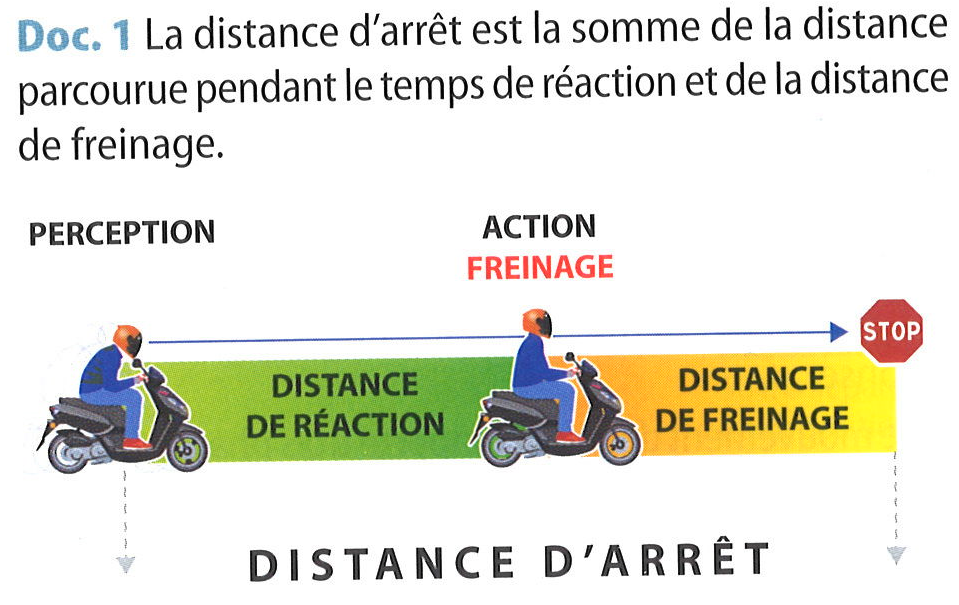
\includegraphics[scale=0.3]{dist_doc1}
	
	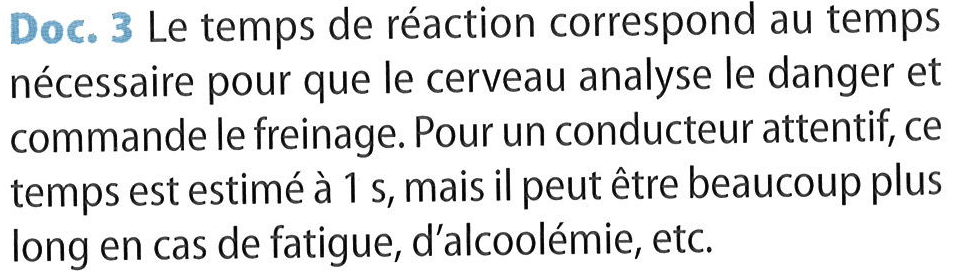
\includegraphics[scale=0.9]{dist_doc3}
	
	
	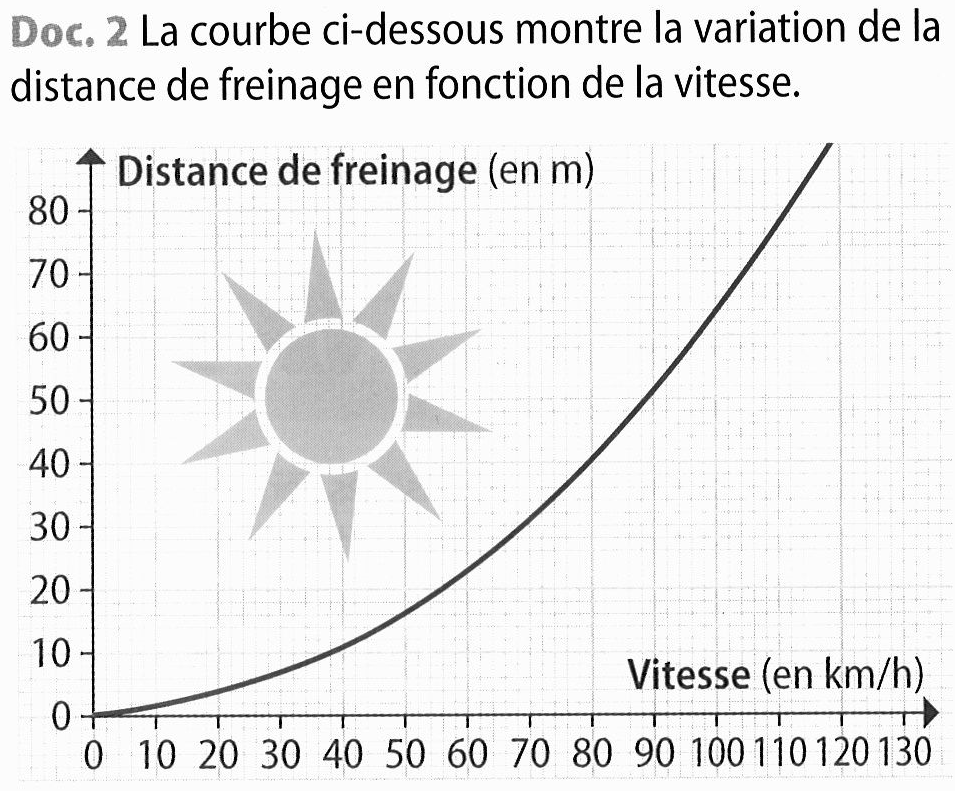
\includegraphics[scale=0.3]{dist_doc2_3}		
\end{multicols}

\begin{questions}
	\question[8] En utilisant les documents ci-dessus, expliquer si Manon peut éviter l'accident.  Détailler le raisonnement, les calculs et comment les documents sont utilisés.
	
	\fillwithdottedlines{12cm}
\end{questions}





